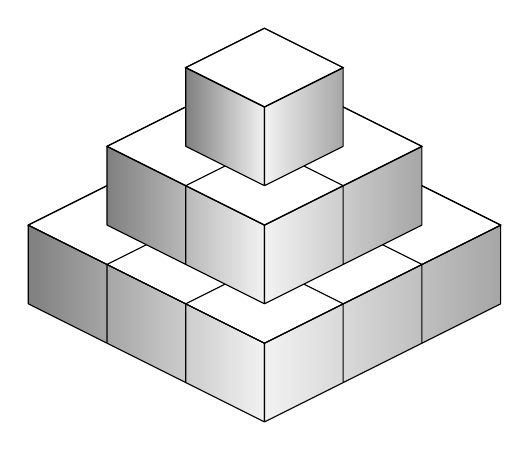
\begin{tikzpicture}
    \tikzset {
        cube layer/.pic = {
            \pgfmathsetmacro{\num}{#1}
            \shade[yslant=-0.5,right color=gray!10, left color=black!50] (0,0) rectangle +(\num,1);
            \draw [yslant=-0.5] (0,0) grid (\num,1);
            \shade[yslant=0.5,right color=gray!70,left color=gray!10] (\num,-\num) rectangle +(\num,1);
            \draw [yslant=0.5] (\num,-\num) grid (2*\num,1-\num);
            \draw [yslant=0.5,xslant=-1,fill=white] (1,1-\num) rectangle +(\num,\num);
            \draw [yslant=0.5,xslant=-1][fill=blue] (1,1-\num) grid (\num+1, 1);
        }
    }
    \path(0, 0) pic {cube layer=3};
    \path(1, 1) pic {cube layer=2};
    \path(2, 2) pic {cube layer=1};
\end{tikzpicture}